\chapter{Introduction}
\label{chap:intro}
\graphicspath{{Introduction/Images/}}

At the dawn of the nineteenth century, Italian astronomer Giuseppe Piazzi was engrossed in observing the Taurus constellation to update a star catalog. On January 1 1801, atop the Palermo observatory in Sicily, he observed a light which wasn't mentioned in the catalog. He followed the strange light for a few more nights, eventually realizing that he had discovered a small planet between Mars and Jupiter. He named the minor planet \textit{Ceres} and it became the first of its kind to be discovered by humans. Broadly speaking, it became the first \textit{asteroid} to ever be discovered \parencite{cunningham2016discovery}. Soon after this discovery, three other minor planets were discovered in the gap between Mars and Jupiter. \textit{Pallas} was discovered in 1802, followed by \textit{Juno} in 1804, and finally \textit{Vesta} in 1807. After the discovery of \textit{Ceres} and \textit{Pallas}, renowned astronomer William Herschel realized that these are a new species of celestial bodies and proposed to call them \textit{asteroids} (which in Greek meant \textit{star-like}) instead of \textit{minor planets}. For nearly 40 years after the discovery of \textit{Vesta}, no additional discoveries were made. Then once again in the second half of the nineteenth century, astronomers started discovering more and more of these asteroids until they realized that there is a whole \textit{belt} of it between Mars and Jupiter \parencite{bottke2002asteroids}.
%
\newline\newline
%
Asteroids are rocky, airless celestial bodies in our Solar System that orbit the Sun and are found in quite large numbers. Relative to the planets, these asteroids are very small and are sometimes even referred to as minor planets. They can be viewed as remnants of the processes that formed the planets of the inner Solar System. Asteroids come in different shapes and sizes, and while most are irregularly shaped, a few are found to be nearly spherical. \Cref{fig:asteroid_shapes} provides a view on the different morphologies of asteroids \parencite{nasa_asteroids_web}. Asteroids are typically classified based on their orbits or put simply, based on their location in the Solar System. Most asteroids are found in the region between Mars and Jupiter, called the \gls{MAB}, and these asteroids are hence called as the \gls{MBO}. Asteroids whose orbit lies close to that of Earth or crosses the Earth's orbit itself are termed as \gls{NEO}.
%%%
\begin{figure}[htb]
\centering
\captionsetup{justification=centering}
    \begin{minipage}{0.48\columnwidth}
        \subfloat[]{
            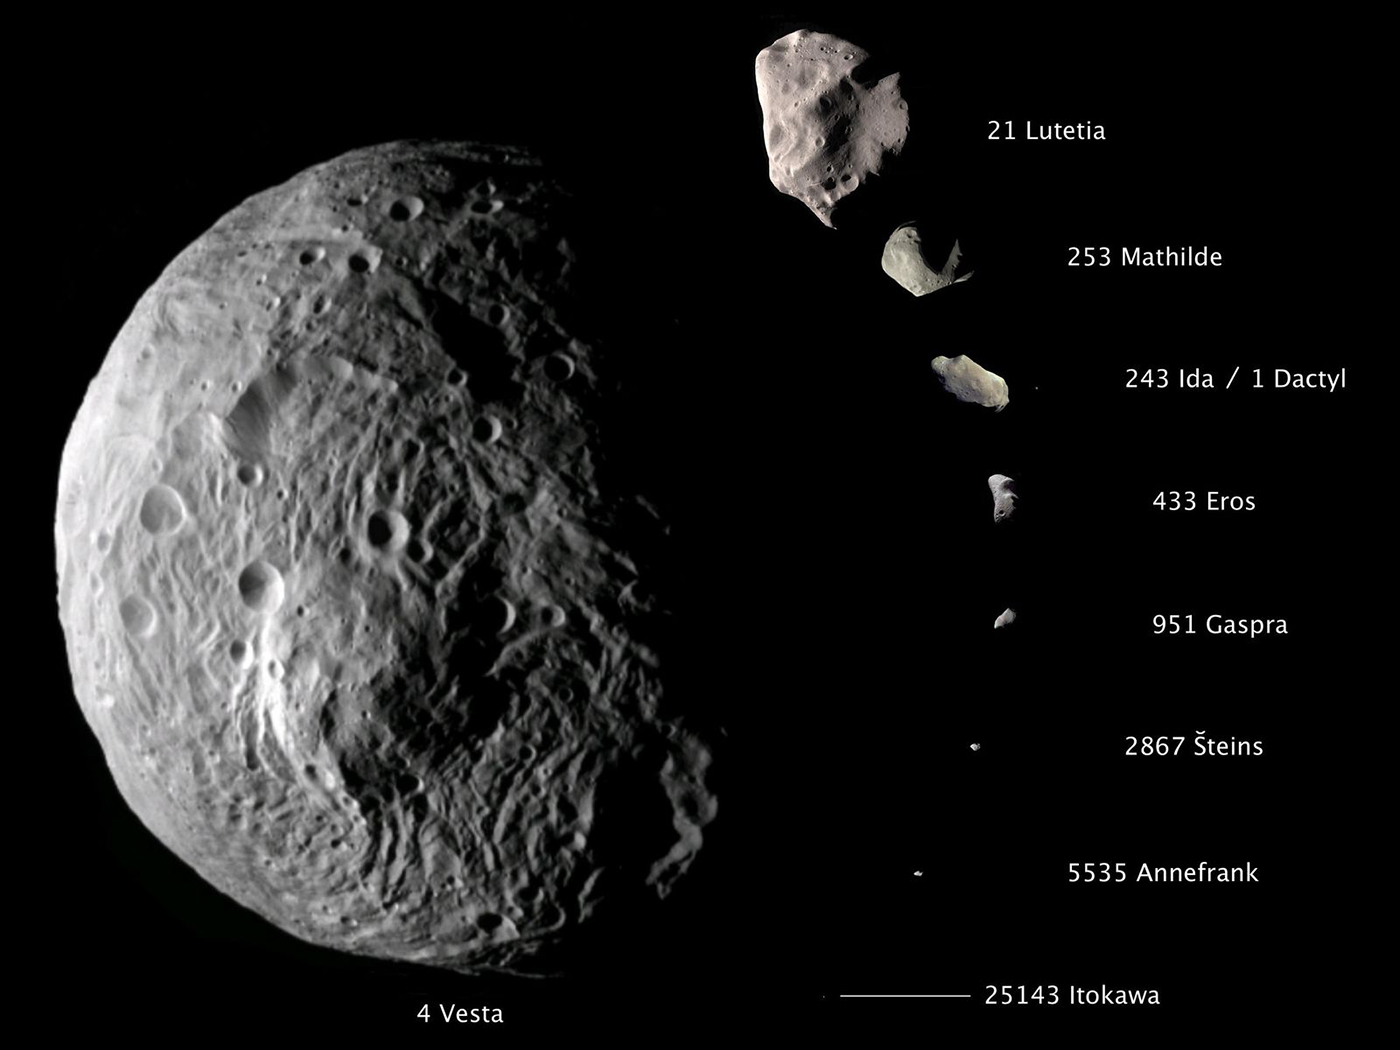
\includegraphics[width=\columnwidth, height=0.5\textheight, keepaspectratio=true]{asteroid_size_comparison.jpg}
            \label{fig:vesta_compared_with_other_asteroids}
        }
    \end{minipage}
    \begin{minipage}{0.48\columnwidth}
        \subfloat[]{
            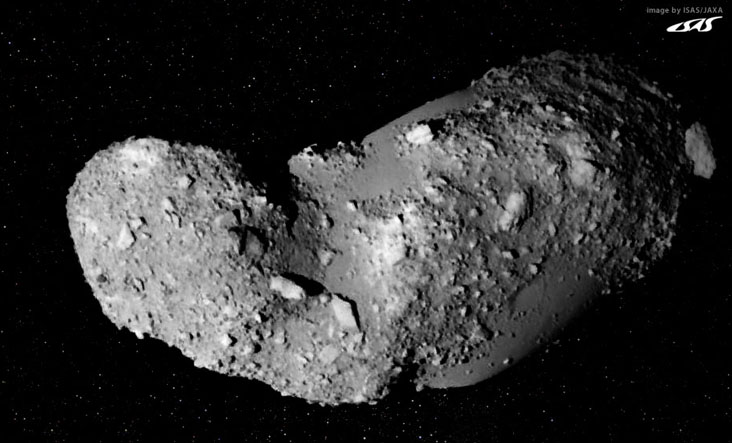
\includegraphics[width=\columnwidth, height=0.25\textheight, keepaspectratio=true]{itokawa.jpg}
            \label{fig:itokawa_image}
        }
        \\[3mm]
        \subfloat[]{
            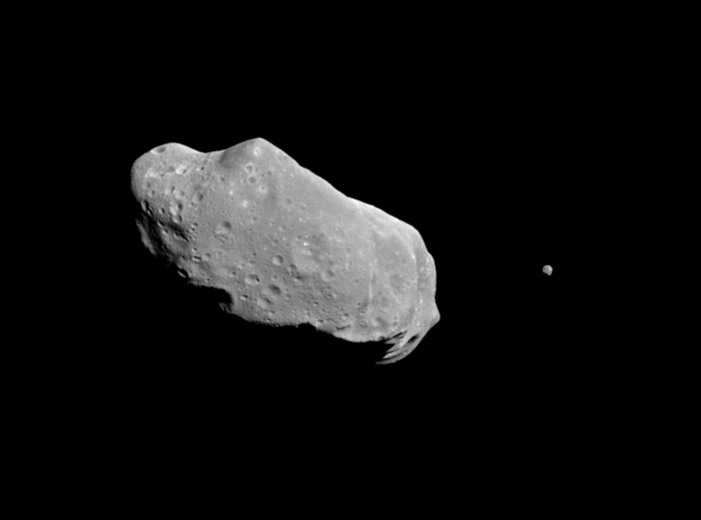
\includegraphics[width=\columnwidth, height=0.25\textheight, keepaspectratio=true]{Ida_Dactyl.jpg}
            \label{fig:ida_dactyl_image}
        }
    \end{minipage}
\caption{Satellite imagery depicting different morphologies of asteroids. \protect\subref{fig:vesta_compared_with_other_asteroids} depicts the size and shape variations amongst a few known asteroids, \protect\subref{fig:itokawa_image} asteroid Itokawa, \protect\subref{fig:ida_dactyl_image} asteroid Ida with its moon Dactyl orbiting around it \parencite{nasa_asteroids_web}.}
\label{fig:asteroid_shapes}
\end{figure}
\FloatBarrier
%%%
% Asteroids are small rocky bodies in our solar system that are orbiting the Sun. These small bodies are basically the remnants from the process that formed the inner planets in our Solar System \parencite{whyAsteroidsWeb}. Asteroids are mainly found in an orbit between Jupiter and Mars and as such are classified as \gls{MBO}. These \gls{MBO} range in size from a few meters to hundreds of kilometers, the largest one being 1 Ceres with a diameter of 948 km. A subset of the \gls{MBO}, called the \gls{NEA}, are asteroids whose orbits come extremely close to, and sometimes even cross, the orbit of the Earth \parencite{jpl_asteroid_web}. Other small bodies in our small system, classified as asteroids when broadly speaking, are the Trojans (small bodies captured at Jupiter's Lagrange points 4 and 5), the \gls{TNO} (small bodies whose orbits around the Sun go beyond Neptune), the Centaurs (small bodies whose orbits lie in between Jupiter and Neptune) \parencite{jpl_asteroid_web}. The asteroids in the main-belt tend to be more rocky in nature, however the small bodies beyond Jupiter tend to have a more icy-composition due to their relatively larger distance from the Sun \parencite{jpl_asteroid_web}.
%
Asteroids don't only exist as single bodies in the Solar System, but they are also found in local multi-body systems consisting of two to even three asteroids. With advanced asteroid detection methods, astrophysicists have found over 190 multiple asteroid systems in the Solar System \parencite{multipleAsteroids}. Contrary to intuition, these multiple asteroid systems exhibit a wide diversity in terms of the size ratios of the components, their mutual orbits and separation, implicating that the individual components evolved differently over time \parencite{multipleAsteroids}. If a multi-asteroid system consists of two or three components, which are bound gravitationally, then it is termed as \textit{binary asteroids} or \textit{triple asteroids} respectively. Triple asteroids are also sometimes termed as \textit{trinary} or \textit{ternary} \parencite{multipleAsteroidsTerminology}. Asteroid components that are not gravitationally bound but are genetically related, are termed as \textit{asteroid pairs}. Asteroid pairs where the larger asteroid is a binary or a triple asteroid, are termed as \textit{paired binaries} or \textit{paired triples}, respectively. The larger component in a binary or triple asteroid system or an asteroid pair, is referred to as the \textit{primary} and similarly the smaller component is referred to as the \textit{secondary} \parencite{multipleAsteroidsTerminology}. Asteroids are further classified based on their dimensions and thermal properties, for which the reader should read the publication in \parencite{multipleAsteroids}.

We now know what asteroids are and the different ways in which they are found in our Solar System, but is it important to study them? There are three major, and most commonly expressed, reasons to study asteroids in our solar system, and not just from a distance such as through radar telescopes placed on Earth, but also through in-situ exploration involving spacecrafts and surface probes. These reasons are mentioned as follows.
\begin{itemize}
\item Asteroids are basically the material left-over from formation of planets in our Solar System. Thus, they are the perfect source to study and understand the origins of the Solar System, as they have remained in the same pristine form since the birth of the Solar System, unlike the planets which have undergone massive topographical and atmospheric changes after their formation. The asteroids can provide valuable information on the chemical composition and initial conditions which led to the formation of planets, including Earth some 4.6 billion years ago. Several scientists have also hypothesized that water and life could have been brought about on Earth through an asteroid or comet and hence exploration of these small bodies could provide a definite answer to an age old question of how life began on Earth \parencite{whyAsteroidsWeb}.
\item Asteroids have been hypothesized to have brought complex molecules to the surface of Earth that eventually resulted in life, but lately they have also been linked to the extinction of dinosaurs due to its impact with Earth. Earth is continuously bombarded with very small interplanetary material, most of which doesn't reach the surface of the Earth but gets evaporated in its atmosphere. However, every few 100 years, an asteroid spanning some tens of meter could impact Earth resulting in widespread damage, in the present case to life and property. But the impact from those will not cause the human race to extinct. But every 100,000 years or so, larger asteroids, spanning over tens of kilometer would impact the Earth, which will lead to extinction of life as we know it now. Although the probability of getting hit by an asteroid on such a large scale is low, it is still a statistical possibility and to be able to device strategies for active deflection of such asteroids, it is imperative that we understand more of the dynamics, properties and composition of the asteroids \parencite{whyAsteroidsWeb}.
\item The third most important reason for us to study asteroids, is the fact that these small bodies are rich in raw materials or minerals. \gls{NEA} can be exploited for the resources that they possess and use it to build space structures or generate fuel for spacecrafts to enable human space exploration in farther reaches of the Solar System. By studying the asteroids, we can develop methods to tap the vast reservoirs of raw materials residing in them \parencite{whyAsteroidsWeb}.
\end{itemize}




